

This theorem doesn't provide 
efficient
algorithms for entailment checking, and this is needed
for parser comparison and integration to be
practical.  Computing the solved forms of $\varphi$ and $\varphi'$ may
be exponential, and the complexity of the {\sc rmrs} validity problem
is unknown.  However, the above theorem illustrates that our
model theory functions in the way it should for parser
comparison and integration, and it can thus be used to prove important
logical properties of shallow parsing systems that adopt {\sc rmrs}.

The outline proof of Theorem~\ref{thm:big-one} is as follows:
\begin{proof}
  ``$\Leftarrow$'': Let $M,\alpha$ an arbitrary model and variable
  assignment that satisfy $\varphi$.  There is a solved form $s$ of
  $\varphi$ such that $M,\alpha \models s$.  By assumption, this means
  that there is a solved form $s'$ of $\varphi'$ such that $s$ is an
  extension of $s'$.  Therefore, $M,\alpha \models s'$ and hence
  $M,\alpha \models \varphi'$.

  ``$\Rightarrow$'': Assume that $\varphi \models \varphi'$, and let
  $s$ be a solved form of $\varphi$.  We need to show that
  we can remove atoms from $s$ such that $s$ remains an extension of
  the resulting $s'$ and $s'$ is a solved form of $\varphi'$.

  We construct $s'$ as the conjunction of all atoms in $s$ that only
  contain variables occurring in $\varphi'$ and all atom $X \dom Y$
  such that $X$ and $Y$ occur in $\varphi'$ and $(X,Y) \in D(s)$.

  It is obvious that $s$ is an extension of $s'$.  Furthermore, $s'$
  is in solved form, because $s$ was a tree and we didn't
  introduce new edges.  The tricky part is to show that $s'$ is a
  solved form of $\varphi'$.  $s'$ contains all labeling atoms of
  $\varphi'$ according to
  Lemma~\ref{lem:entailment-preserves-labeling-atoms}; a similar
  argument holds for inequality atoms.  Finally, $D(\varphi')
  \subseteq D(s')$ because $M,\alpha \models s'$ and $s'$ is
  tree-shaped and normal and therefore contains all dominance statements
  that are true in $M$.
\end{proof}

\begin{lemma} \label{lem:entailment-preserves-labeling-atoms}
  Under the assumptions of
  Theorem~\ref{thm:big-one}, if $\varphi \models
  \varphi'$, then $\varphi'$ only contains labeling atoms that also
  occur in $\varphi$.  
\end{lemma}
\begin{proof}
  Let $\varphi \models \varphi'$, but let $\varphi'$ contain a
  labeling atom $X \Neq f(X_1,\ldots,X_n)$ that doesn't occur in
  $\varphi$.  Call this atom $A$.

  Furthermore, let $M,\alpha \models \varphi$ arbitrary.  Because
  $M,\alpha \models \varphi'$, we must have $M(\alpha(X)) = f$.

  Now replace the label of $\alpha(X)$ in $M$ by some other symbol $g$
  of arity $n$.  Call the resulting model $M'$.  We still have
  $M',\alpha \models \varphi$ because $\varphi$ doesn't contain a
  labeling atom for $X$.  But now $M',\alpha \not\models \varphi'$.
  This contradicts the entailment assumption.
\end{proof}

It is really necessary to state
Theorem~\ref{thm:big-one} in terms of extensions of
solved forms.  It is \emph{not} true that $\varphi \models \varphi'$
implies that $\varphi$ is an extension of $\varphi'$.  A
counterexample is shown in Fig.~\ref{fig:counterexample}, where the
right-hand constraint entails the left-hand constraint (they are
equivalent), but is not an extension of it.

\begin{figure}
  \centering
  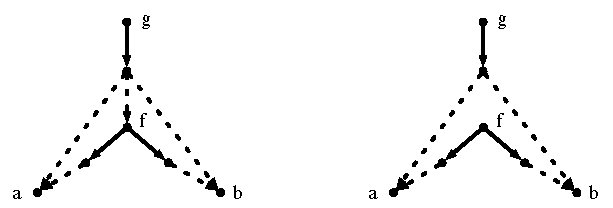
\includegraphics[scale=0.6]{pic-extension-counterexample}
  \caption{A counterexample to a simpler version of Theorem~\ref{thm:big-one}.}
  \label{fig:counterexample}
\end{figure}

